%\documentclass{article}[10pt,a4paper]
%\usepackage{amsfonts, amsmath, amssymb}
%\usepackage[margin=1in]{geometry}
%\usepackage{graphicx, subcaption}

\begin{answer}
	
	\begin{figure}[H]
		\centering
		\begin{subfigure}[H]{0.45\linewidth}
			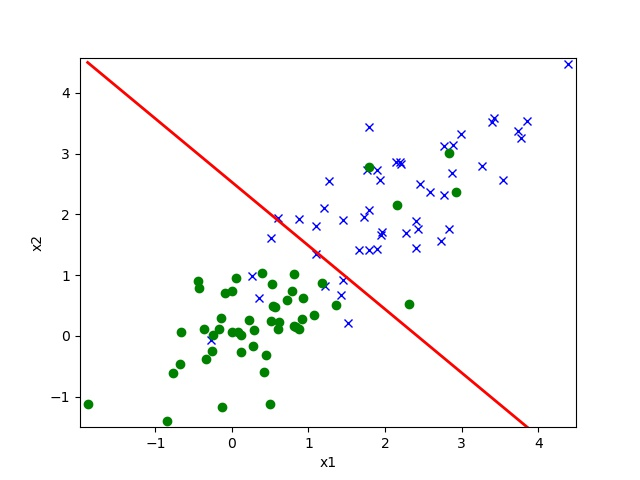
\includegraphics[width=\linewidth]{logreg_2}
			\caption{Logistic regression}
		\end{subfigure}
		\begin{subfigure}[H]{0.45\linewidth}
			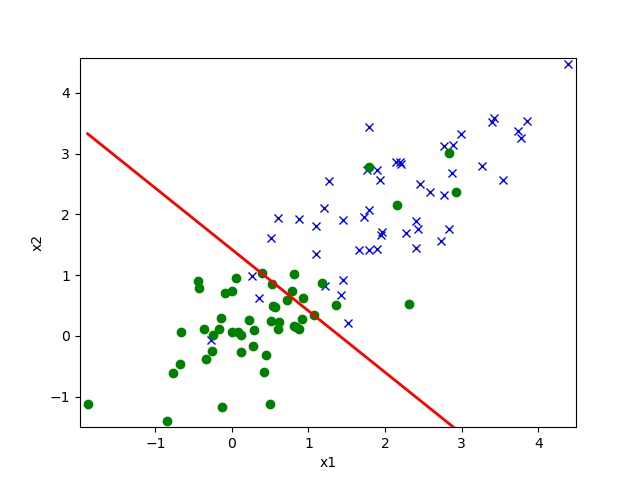
\includegraphics[width=\linewidth]{gda_2}
			\caption{GDA}
		\end{subfigure}
		\caption{Results on the Dataset 2.}
	\end{figure}
	In the validation data set 2, both models gave rather similar results, though the logistic regression model was slightly better. Overall, both learned decision boundaries are good on this data set. \\
	As we have observed from the previous question, GDA performed worse than logistic regression on data set 1. Two classes in data set 2 don't look like Gaussian distributed.
	
\end{answer}

